\chapter{Implementation Details}
\label{chap:ch5}

\quad This chapter details the architecture used, detailing the design, and discussing the implementation specifics.

\section{Architechure}

\quad The tool is a web application, specifically a Chrome extension, named "Depression Signs Detector" and has the icon showed in Figure \ref{depressionsSignsDetectorIcon}, which has a minimalist design showing a heart which has as the left part a brain, showing the importance of mental health. The developed tool's backend operates locally, and the frontend is configured in developer mode as a Chrome extension.

It adheres to the REST software architectural design. RESTful Web Services facilitate communication with the client through the receipt of HTTP methods such as GET, POST, PUT, DELETE, accompanied by some additional data, and respond with the precise data needed for the client to display information to the user. The response format is typically JSON (JavaScript Object Notation), although XML is also possible. This web application is divided into two main servers: the frontend and the backend.

\begin{figure}[htbp]
	\centering
		
\includegraphics[scale=0.1]{LaTeX Bachelor Thesis Depression Signs Detection/figures/icon1024.png}
	\caption{Depression Signs Detector Icon}
	\label{depressionsSignsDetectorIcon}
\end{figure}

\section{Backend}

\quad The backend serves as the data access layer of an application. Typically, it accesses the database to fetch data and carries out various computations with this data. However, in this specific application, there is no database layer since there is no requirement for data storage. Here, the backend is facilitated by a Python webserver, constructed using Flask. Flask is recognized as a lightweight micro web application framework for Python \cite{ronacher2021flask}, selected for its straightforward configuration and the freedom it offers in architectural choices, such as the absence of a database. Unlike more comprehensive Python web frameworks like Django, Flask does not provide a database abstraction layer, form validation, or other extensive libraries. The choice of Flask over other frameworks was influenced by the simplicity it brings to server management.

\begin{figure}[htbp]
	\centering
		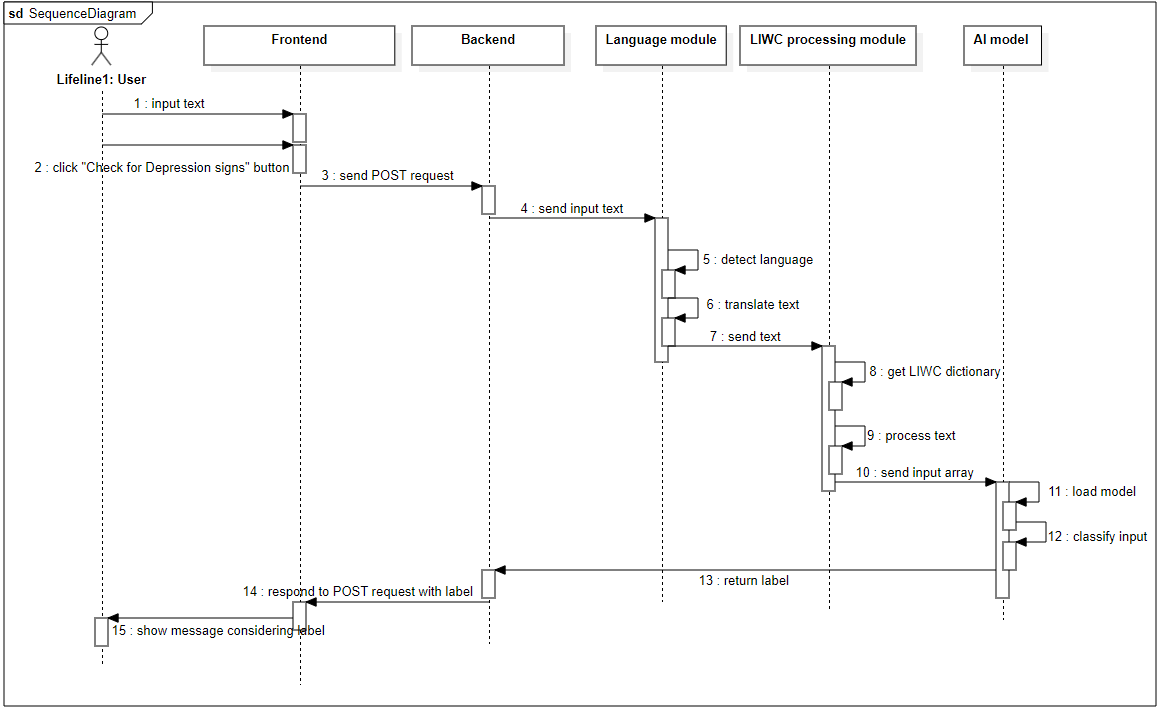
\includegraphics[scale=0.5]{LaTeX Bachelor Thesis Depression Signs Detection/figures/SequnceDiagram.png}
	\caption{Sequence Diagram for Detecting Signs of Depression}
	\label{seqDiag}
\end{figure}

The only role of the backend in this application is to handle a POST request which is annotated with "/classify" containing the input text in its body, and to respond with a 1 if the AI model determines that the text is indicative of a depressed individual, and a 0 otherwise. Firstly the input text in the body of the POST request, used for security reasons instead of GET, is checked in the Language module, showed in Figure \ref{seqDiag}. With the help of googlelib \cite{googletranslib}, which also has a detect language functionality, it is seen whether the received text is in Romanian or English. If not, we translate it into English.

Considering the language the text is in after the language module, an LIWC dictionary is selected, namely for English "LIWC-22" and for Romanian "Ro-LIWC-2015". Then, the text is processed in python with the help of the CLI provided by LIWC and the output is received in cmd as seen in Figure \ref{codeLiwcCli}.

\begin{figure}[htbp]
	\centering
		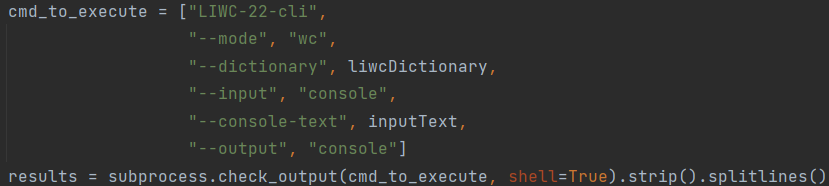
\includegraphics[scale=0.5]{LaTeX Bachelor Thesis Depression Signs Detection/figures/codeLiwcCLI.png}
	\caption{Python Code to Process Text Using LIWC CLI }
	\label{codeLiwcCli}
\end{figure}

Once more, based on the language of the text, the appropriate AI model, either Romanian or English, is loaded. This model is then used to classify the text, and the label is sent back to the frontend, illustrated in Figure \ref{seqDiag}.

\section{Frontend}

\quad The frontend of this application is developed using the React JavaScript library and TypeScript. As seen in the Figure \ref{interface}, it containts a text box where the text to be classified is to be put and a button for initiating the POST request. After receiving the response from backend containing the label predicted by the classifier, two messages can be shown:
\begin{itemize}
    \item label 0 (no depression detected): It appears there are no signs of depression, which is reassuring. Thank you for taking the time to look out for the well-being of the person who wrote this message.
    \item label 1 (depression detected):  Signs of depression detected. It might be helpful to reach out and talk more with the person who wrote this message. Offering a listening ear can make a big difference.
\end{itemize}

\begin{figure}[htbp]
	\centering
		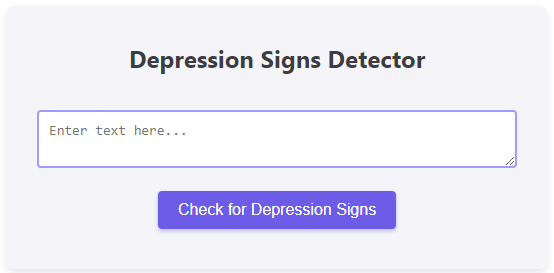
\includegraphics[scale=0.5]{LaTeX Bachelor Thesis Depression Signs Detection/figures/interface.png}
	\caption{Chrome Extension User Interface}
	\label{interface}
\end{figure}








